\chapter{Finite Difference Method} \index{Finite Difference Method|(}

\section{Introduction} \label{sec:fdm_intro}

The Finite Difference Method\index{Finite Difference Method} is well suited to study $z$-invariant
devices, where $z$ is the direction of propagation of the
electromagnetic field, like the one shown in \figref{fig:fdm_waveguide}.

\begin{figure}[htbp]
  \begin{center}
    \resizebox{6cm}{!}{\input{pics/fdm_waveguide.pdf_t}}
  \end{center}
  \caption{$z$-invariant waveguide with a generic cross section.}
  \label{fig:fdm_waveguide}
\end{figure}

Maxwell equations, without sources, in the harmonic regime, for a
linear non-magnetic medium, read \cite{someda_electromagnetic}:
\begin{equation} \label{eqn:fdm_maxwell} \begin{cases}
    \Rot{\E} = -\imath \omega \mu_0 \H \\
    \Rot{\H} = \imath \omega \epsilon \E
\end{cases} . \end{equation}

From the second equation we can write $\E = \frac{1}{\imath
\omega \epsilon} \Rot{\H}$ and obtain the Helmholtz
equation for the $\H$ field:
\begin{equation} \label{eqn:fdm_helmholtz_h}
  \Rot{\frac{1}{\epsilon} \Rot{\H}} - \omega^2 \mu_0 \H = 0.
\end{equation}

The same can be done for the $\E$ field, obtaining:
\begin{equation} \label{eqn:fdm_helmholtz_e}
  \Rot{\Rot{\E}} - \omega^2 \mu_0 \epsilon \E = 0.
\end{equation}

Where $\epsilon$ is homogeneous, from Helmholtz equation we obtain the
Laplace equation, valid for both $\H$ and $\E$ fields:
\begin{equation} \label{eqn:fdm_laplace}
  \Lap{\Vector{F}} + \omega^2 \mu_0 \epsilon \Vector{F} = 0,
\end{equation}
where $\Vector{F} = \bigl\{ \begin{smallmatrix} \H \\ \E \end{smallmatrix}
\bigr\}$ and we have used $\Rot{\Rot{\bullet}} = \Grad{\Div{\bullet}} -
\Lap{\bullet}$ and $\Div{\Vector{F}} = 0$ (i.e. $\Div{\H} = 0$ or
$\Div{\E} = 0$).

Now, a $z$-dependence of the type $e^{-\imath \beta z}$ is supposed
for both $\E$ and $\H$: this is the $z$-dependence of any solution of
the wave equation in a translational symmetric system in the $z$
direction. Moreover, any mode can be described simply by its
transversal coordinates $x$ and $y$
\cite{someda_electromagnetic}. Therefore, in Cartesian coordinates,
where $\H = \left( H_x,H_y,H_z \right)$ and $\E = \left( E_x,E_y,E_z
\right)$, Laplace equation \eqref{eqn:fdm_laplace} becomes:
\begin{equation} \label{eqn:fdm_laplace_cartesian} \begin{cases}
    \pdx^2 F_x + \pdy^2 F_x + (\omega^2 \mu_0 \epsilon - \beta^2) F_x = 0 \\
    \pdx^2 F_y + \pdy^2 F_y + (\omega^2 \mu_0 \epsilon - \beta^2) F_y = 0
\end{cases} , \end{equation}
where, again, $F$ stands for $H$ or $E$.

Note that $F_x$ and $F_y$ are decoupled. Coupling between the two
transverse components only arises where $\epsilon$ is non-homogeneous
and it's stronger where bigger changes in $\epsilon$ are present. This
can be easily seen also theoretically: in low index contrast devices
modes are \emph{almost purely} TE or TM, while in high index contrast
devices they are \emph{quasi}- TE or TM. See \parref{par:hic_devices}.

Helmholtz equations \eqref{eqn:fdm_helmholtz_h} and
\eqref{eqn:fdm_helmholtz_e}, alone, are not equivalent to Maxwell
equations: they have solutions that are not solutions of Maxwell
equations, which are called \emph{spurious solutions}. To avoid them,
a supplementary condition must be imposed: $\Div{\H} = 0$ (or
$\Div{\D} = 0$). This can be noted taking the divergence of
\eqref{eqn:fdm_helmholtz_h} (or \eqref{eqn:fdm_helmholtz_e}): it is
clear that, without this condition, an arbitrary field $\H$ (or $\E$),
even if non-divergenceless, would be a zero frequency solution. This is,
obviously, unphysical, because the divergenceless condition must hold
for all frequencies.

Other approximations can be imposed to the previous equations, to
reduce the complexity of the problem and simplify the algorithm to
implement on a computer. The most often used simplification, is to
suppose that TE and TM polarization are decoupled: the resulting
algorithm is the so called \emph{semivectorial}, described in
\secref{sec:semivectorial_mode_solver}. It is very easy to implement
and very effective to study low index contrast devices. Unluckily, to
study high index contrast devices, such as polarization rotators (see
\charef{cha:polrot}), a fully vectorial mode solver\index{Mode!solver!vectorial} is needed, which
takes into account the TE/TM coupling. It is described in
\secref{sec:vectorial_mode_solver}.

\section{Semivectorial Mode Solver} \index{Mode!solver!semivectorial|(} \label{sec:semivectorial_mode_solver}

The semivectorial mode solver that we have implemented is a very simple,
yet accurate, method, which can be used to have a first insight into
the problem, when an absolute accuracy is not needed. It is based on
the algorithm described in \cite{stern_semivectorial}.

\begin{figure}[htbp]
  \begin{center}
    \resizebox{6cm}{!}{\input{pics/stern_fig1.pdf_t}}
  \end{center}
  \caption{Typical ridge waveguide, with a cladding, a guiding layer
    and a substrate. The reference system is also shown.}
  \label{fig:stern_fig1}
\end{figure}

Ridge waveguides like the one in \figref{fig:stern_fig1} can be studied: the
refractive index profile precludes an analytical solution which is,
strictly speaking, fully vectorial. In fact, TE and TM polarizations
can not be distinguished: as pointed out in the
\secref{sec:fdm_intro}, this is particularly true the higher the
refractive index discontinuities are.

The simplicity of the present method, which is both its strength and
its weakness, derives from some hypothesis on the
geometry and the physics of the problem:
\begin{enumerate}
\item
  the refractive index is piecewise constant inside the domain, with the
  discontinuities occurring only at horizontal or vertical
  planes\footnote{The algorithm is implemented in Cartesian coordinates.};
\item
  TE and TM polarizations are considered as decoupled, instead of
  being coupled into a fully vectorial solution: this allows to
  formulate two separate eigenproblems, one for each polarization, of
  smaller dimension than the full vectorial problem, but introduces
  the already mentioned approximations.
\end{enumerate}

Starting from Maxwell equations in the frequency domain for a linear
sourceless medium, we have:
\begin{equation} \label{eqn:stern_maxwell} \begin{cases}
  \Rot{\E} = -\imath \omega \mu \H \\
  \Rot{\H} = \imath \omega \epsilon \E \\
\end{cases} \end{equation}
and electric and magnetic Gauss laws:
\begin{equation} \label{eqn:stern_gauss} \begin{cases}
  \Div{\D} = 0 \\
  \Div{\B} = 0
\end{cases} . \end{equation}

Combining them together, we obtain Helmholtz equation for the electric
field:
\begin{equation} \label{eqn:stern_toward_helmholtz}
\Rot{\Rot{\E}} = \Grad{\Div{\E}} - \Lap{\E} = \omega^2 \epsilon \mu \E = k^2 \E.
\end{equation}

The first hypothesis leads to the first simplification. Inside the
regions where the refractive index is constant, from the first
equation in \eqref{eqn:stern_gauss}, we have:
\begin{equation*}
\Div{\D} = \Div{\left( \epsilon \E \right)} = \DotProd{\Grad{\epsilon}}{\E} +
\epsilon \Div{\E} = 0,
\end{equation*}
from which we can write:
\begin{equation*}
\Div{\E} = \DotProd{\frac{\Grad{\epsilon}}{\epsilon}}{\E}.
\end{equation*}

Where $\epsilon$ is piecewise constant, $\Grad{\epsilon} = 0$ and
$\Div{\E} = 0$ is satisfied: elsewhere, this is not strictly true, but
the smaller the gradient, the smaller the refractive index
discontinuities and the less important this approximation.

With this hypothesis, \eqref{eqn:stern_toward_helmholtz} becomes:
\begin{equation} \label{eqn:stern_helmholtz}
\Lapt{\E} + k^2 \E = \beta^2 \E,
\end{equation}
where we have supposed a $z$ dependence of the $\E$ fields of the
type $e^{-\imath \beta z}$ and $\Lapt{} \eqdef \pdx^2 + \pdy^2$.

\eqref{eqn:stern_helmholtz} does not contain any coupling between
the $x$ and $y$ components of the $\E$ field, therefore it holds
independently for each polarization:
\begin{align} \label{eqn:stern_helmholtz_decoupled}
\Lapt{\E} + k^2 \E = \beta^2 \E && \Rightarrow &&
\begin{cases}
  \Lapt{E_x} + k^2 E_x = \beta^2 E_x \\
  \Lapt{E_y} + k^2 E_y = \beta^2 E_y
\end{cases} . \end{align}

We use now the second hypothesis: for the TE polarization, the
electric field is $\E = (E_x,0,E_z)$ and the first equation in
\eqref{eqn:stern_helmholtz_decoupled} holds; for the TM polarization,
$\E = (0,E_y,E_z)$ and the second holds.

Helmholtz equations \eqref{eqn:stern_helmholtz_decoupled} must now be
discretized somehow, to be able to solve them on a
computer. Discretization is done substituting the second order
derivatives by finite differences on an orthogonal grid, like the one
in \figref{fig:stern_fig2}. Each internal interface is placed half-way
between adjacent grid lines and each internal grid point is placed at
the center of a rectangular cell of constant refractive
index. Refractive index changes are only allowed at cell boundaries.

\begin{figure}[htbp]
  \begin{center}
    \resizebox{6cm}{!}{\input{pics/stern_fig2.pdf_t}}
  \end{center}
  \caption{Cell structure (in dashed lines) of the finite difference
    grid (in solid lines): refractive indices are constant
    within each cell, with discontinuities only allowed at cell
    boudaries. Cells have dimensions $\deltax \times \deltay$.}
  \label{fig:stern_fig2}
\end{figure}

On the domain boundaries, we can impose different conditions:
\begin{itemize}
\item
  \emph{Perfect Electric Conductor} (PEC): null tangential $\E$ and
  $\partial_n \E$, with $\Versor{n}$ versor normal to the boundary;
\item
  \emph{Perfect Magnetic Conductor} (PMC): null tangential $\H$ and
  $\partial_n \H$, with $\Versor{n}$ versor normal to the boundary;
\item
  \emph{Perfectly Matched Layers} (PMLs) or \emph{Transparent Boundary
  Conditions} (TBC) to simulate free space.
\end{itemize}

For the TE polarization, the second order discretization of the space
derivatives reads:
\begin{equation} \label{eqn:stern_discretization} \begin{aligned}
\deltax^2 \left( \pdx^2 E_x \right)^{(P)}_{r,s} & \simeq 2 K^{(W)}_{r-1,s} E_{r-1,s} \\
  & - \left[ 2 + \left( K^{WP}_{r,s} - K^{W}_{r-1,s} \right) + \left(
  K^{EP}_{r,s} - K^{E}_{r+1,s} \right) \right] E_{r,s} \\
  & + 2 K^{(E)}_{r+1,s} E_{r+1,s} \\
\deltay^2 \left( \pdy^2 E_x \right)^{(P)}_{r,s} & \simeq E_{r,s-1} - 2 E_{r,s} + E_{r,s+1} .
\end{aligned} \end{equation}

Note that the $E_x$ component is continuous across horizontal
interfaces and discontinuous across vertical interfaces. Factors $K$
are defined:
\begin{align*}
K^{(E)}_{r+1,s}  & \eqdef \frac{k^2_{r+1,s}}{k^2_{r,s} + k^2_{r+1,s}} \\
K^{(EP)}_{r+1,s} & \eqdef \frac{k^2_{r,s}}{k^2_{r,s} + k^2_{r+1,s}} \\
K^{(W)}_{r-1,s}  & \eqdef \frac{k^2_{r-1,s}}{k^2_{r-1,s} + k^2_{r,s}} \\
K^{(WP)}_{r+1,s} & \eqdef \frac{k^2_{r,s}}{k^2_{r-1,s} + k^2_{r,s}} .
\end{align*}

Substituting of \eqref{eqn:stern_discretization} into
\eqref{eqn:stern_helmholtz_decoupled} and letting $\Matrix{E}_{TE}$ be
the column vector with all the $E_x$ values, one for each node of the
discretization grid, we can write the matricial eigenvalue equation:
\begin{equation} \label{eqn:stern_eigenproblem}
\Prod{\Matrix{A}_{TE}}{\Matrix{E}_{TE}} = \beta^2_{TE} \Matrix{E}_{TE}.
\end{equation}

The order in which the $E_x$ values are stored in the
$\Matrix{E}_{TE}$ vector is arbitrary: the problem is not dependent on
the particular numbering of the grid nodes. Efficiency of numerical
methods used to solve the eigenvalue problem
\eqref{eqn:stern_eigenproblem} depends on the numbering, though: for
example, the ILU decomposition of the sparse matrix $\Matrix{A}_{TE}$
tend to be more efficient if its non-zero values are closer to the
main diagonal. Thus, any node numbering satisfying this condition is
preferred in this case: luckily, most numerical routines to solve
eigenvalue problems internally reorder $\Matrix{A}_{TE}$ to achieve
better results.

A very similar reasoning can be applied to the TM polarization, for which
the $E_y$ component is continuous across vertical interfaces and
discontinuous across horizontal interfaces. We end up with a
matricial equation very similar to \eqref{eqn:stern_eigenproblem}:
\begin{equation*}
\Prod{\Matrix{A}_{TM}}{\Matrix{E}_{TM}} = \beta^2_{TM} \Matrix{E}_{TM}
\end{equation*}
that can be solved in the same way.

\index{Mode!solver!semivectorial|)}

\section{Vectorial Mode Solver} \index{Mode!solver!vectorial|(} \label{sec:vectorial_mode_solver}

As said in \secref{sec:semivectorial_mode_solver}, a semivectorial
mode solver is not accurate enough to study HIC devices: hence, we have
implemented a fully vectorial mode solver.

The algorithm chosen is the one presented in \cite{lusse_analysis},
that we are going to analyze more in detail here. Based on the Finite
Difference approach, it is well known to ensure the absence of
spurious modes, by a proper formulation of the physical equations and
of the boundary conditions. It has also been proven to achieve a
considerable precision on the computed effective index\index{Effective!index}. This is a key
point in today's designs: hundreds of microns long devices are quite common
and errors on the effective indices as small as $10^{-5}$ at optical
frequencies ($\lambda = 1.5 \mu m$) results in a very high overall
phase error.

\begin{figure}[htbp]
  \begin{center}
    \resizebox{6cm}{!}{\input{pics/lusse_fig2.pdf_t}}
  \end{center}
  \caption{Non-uniform Cartesian mesh for the vectorial mode solver.}
  \label{fig:lusse_fig2}
\end{figure}

Let's consider a $z$-invariant waveguide and discretize its $xy$ cross
section with a non-uniform Cartesian mesh, like in
\figref{fig:lusse_fig2}. Association of physical quantities to
geometrical elements is done supposing the magnetic field $\H$
attached to the nodes of the mesh and the refractive index constant
inside each rectangle of the mesh: therefore, discontinuities can only
occur at the edges. As said to deduce \eqref{eqn:fdm_laplace}, inside
each rectangle of the mesh, the decoupled version of the Helmholtz
equation holds. Let's call $\Evaluate{H}{W} = H_W$ the magnetic field
evaluated at point $W$ (a similar nomenclature holds for $P$, $N$, $S$
and $E$) and expand it in Taylor series around the point
$P$ to obtain a discretized form of $\partial_x^2 H_W$:
\begin{align}
  H_W & = H_P + \pdx H|_w (-w) + \frac{1}{2} \pdx^2 H|_w (-w)^2 + \BigO{w^3}, \notag \\
\intertext{therefore:}
  \pdx^2 H|_w & = \frac{2 H_W}{w^2} - \frac{2 H_P}{w^2} + \frac{2}{w} \pdx H|_w + \BigO{w^3}. \label{eqn:lusse_partial}
\end{align}

Analogous expressions hold for $H_S$, $H_E$, $H_N$ and for
$\pdy^2$. Note that the first order derivatives are not discretized:
the reason will be clear after the discussion about the boundary
conditions.

Substituting \eqref{eqn:lusse_partial} into
\eqref{eqn:fdm_laplace_cartesian}, we obtain the discretized form,
for both $H_x$ and $H_y$:
\begin{equation} \label{eqn:lusse_helmholtz} \begin{aligned}
  \frac{2 H_W}{w^2} - \frac{2 H_P}{w^2} + \frac{2}{w} \pdx H|_w +
  \frac{2 H_N}{w^2} - \frac{2 H_P}{w^2} + \frac{2}{w} \pdx H|_n +
  \epsilon_1 k^2 H_P & = \beta^2 H_P \\
  \frac{2 H_W}{w^2} - \frac{2 H_P}{w^2} + \frac{2}{w} \pdx H|_w +
  \frac{2 H_S}{w^2} - \frac{2 H_P}{w^2} + \frac{2}{w} \pdx H|_s +
  \epsilon_2 k^2 H_P & = \beta^2 H_P \\
  \frac{2 H_E}{w^2} - \frac{2 H_P}{w^2} + \frac{2}{w} \pdx H|_e +
  \frac{2 H_S}{w^2} - \frac{2 H_P}{w^2} + \frac{2}{w} \pdx H|_s +
  \epsilon_3 k^2 H_P & = \beta^2 H_P \\
  \frac{2 H_E}{w^2} - \frac{2 H_P}{w^2} + \frac{2}{w} \pdx H|_e +
  \frac{2 H_N}{w^2} - \frac{2 H_P}{w^2} + \frac{2}{w} \pdx H|_n +
  \epsilon_4 k^2 H_P & = \beta^2 H_P.
\end{aligned} \end{equation}

The condition of divergenceless $\H$ is imposed through the boundary
conditions. $H_z$ and $E_z$ are both continuous everywhere on the $xy$
plane; therefore:
\begin{align} \label{eqn:lusse_continuity_hz}
\Div{\H} = 0 && \Rightarrow && H_z = \frac{1}{\imath \beta} \left( \pdx H_x + \pdy H_y \right)
\end{align}
and, from the second of Maxwell equations \eqref{eqn:fdm_maxwell}:
\begin{align} \label{eqn:lusse_continuity_ez}
  \Rot{\H} = \imath \omega \epsilon \E && \Rightarrow && E_z = \frac{1}{\imath \omega \epsilon} \left( \pdx H_y - \pdy H_x \right)
\end{align}

Discontinuities of $\epsilon$ can only occur on the edges of the
mesh, so the boundaries between two different values of $\epsilon$ can be:
\begin{enumerate}
\item
  horizontal boundaries: on which $H_x$ and $H_z$ are continuous, and
  \ref{eqn:lusse_continuity_hz} becomes:
  \begin{equation*}
    \dy H_y|_n = \dy H_y|_s,
  \end{equation*}
  while, \ref{eqn:lusse_continuity_ez} becomes:
  \begin{equation*}
    \epsilon_n \dy H_x|_s - \epsilon_s \dy H_x|_n = (\epsilon_n - \epsilon_s) \dy H_x;
  \end{equation*}
\item
  vertical boundaries: on which $H_y$ and $H_z$ are continuous, and
  \ref{eqn:lusse_continuity_hz} and \ref{eqn:lusse_continuity_ez} become,
  respectively:
  \begin{equation*}
    \pdx H_x|_w = \pdx H_x|_e
  \end{equation*}
  and
  \begin{equation*}
    \epsilon_e \pdx H_y|_w - \epsilon_w \pdx H_y|_e = (\epsilon_e - \epsilon_w) \pdx H_y.
  \end{equation*}
\end{enumerate}

With these four boundary conditions and \eqref{eqn:lusse_helmholtz},
the requested coupled differential equations in $H_x$ and $H_y$ can be
obtained. Just note that, for the $H_x$ component, multiplying the
first of \eqref{eqn:lusse_helmholtz} by $\epsilon_2 n/2$ and summing
it to the second multiplied by $\epsilon_1 s/2$, we obtain the left
hand side of the second boundary condition. Similar arithmetical
manipulations can be done, to obtain all the terms in the boundary
conditions and to eliminate the first order derivative in
\ref{eqn:lusse_helmholtz}.  Finally, two coupled equations in $H_x$
and $H_y$ can be written, in the form:
\begin{equation*} \begin{cases}
    a_{xxW} H_{xW} + a_{xxE} H_{xE} + a_{xxN} H_{xN} + a_{xxS} H_{xW}
    + a_{xxP} H_{xP} + \\
    a_{xyW} H_{yW} + a_{xyP} H_{yP} + a_{xyE} H_{yE} = \beta^2 H_{xP} \\
    a_{yyW} H_{yW} + a_{yyE} H_{yE} + a_{yyN} H_{yN} + a_{yyS} H_{yW}
    + a_{yyP} H_{yP} + \\
    a_{yxW} H_{xW} + a_{yxP} H_{xP} + a_{yxE} H_{xE} = \beta^2 H_{yP}
\end{cases} . \end{equation*}

In a more compact matricial form:
\begin{equation*}
  \Prod{\Matrix{A}}{\Matrix{H}} = \Prod{
    \begin{bmatrix}
      \Matrix{A}_{xx} & \Matrix{A}_{xy} \\
      \Matrix{A}_{yx} & \Matrix{A}_{yy}
    \end{bmatrix}
  }{
  \begin{bmatrix}
      \Matrix{H}_x \\
      \Matrix{H}_y
  \end{bmatrix}} = \beta^2
  \begin{bmatrix}
      \Matrix{H}_x \\
      \Matrix{H}_y
  \end{bmatrix} = \beta^2 \Matrix{H},
\end{equation*}
where $\Matrix{A_{ij}}$ contains all the coefficients
$a_{ij,rs}$\footnote{The explicit value of the coefficients
$a_{ij,rs}$ can be found in \cite{lusse_analysis}.}, $i,j = x,y$, and
$\Matrix{H}_x$ ($\Matrix{H}_y$) all the $x$ ($y$) components of the
magnetic field, one for each grid point. Note that the coupling
between $H_x$ and $H_y$ is caused by the elements of the off-diagonal
matrices $\Matrix{A}_{xy}$ and $\Matrix{A}_{yx}$: in semivectorial
algorithms or in homogeneous regions, they are zero.

\index{Mode!solver!semivectorial|)}

\section{Examples and validation}

As an example of a typical device that can be studied with the described
mode solvers, consider the rib waveguide presented in \cite{lohmeyer_wmm}.

The domain is shown in \figref{fig:rib}, where: $n_s = 3.34$, $n_f =
3.44$, $n_c = 1.0$, $w = 2 \mu m$, $h = 1.1 \mu m$ and $t = 0.2 \mu m$.

\begin{figure}[htbp]
  \begin{center}
    \resizebox{4cm}{!}{\input{pics/rib.pdf_t}}
  \end{center}
  \caption{Rib waveguide profile, taken from \cite{lohmeyer_wmm}.}
  \label{fig:rib}
\end{figure}

In \figref{fig:wmm1_stern} and \figref{fig:wmm1_lusse}, results are
shown for both the algorithms, the semivectorial of
\secref{sec:semivectorial_mode_solver} and the fully vectorial of
\secref{sec:vectorial_mode_solver}, respectively. The first four
guided modes are plotted, two TE and two TM. The accordance between
the two algorithms, in this case, is very good (see
\tabref{tab:wmm1}), within $0.02\%$. They also agree with the results
reported in \cite{lohmeyer_wmm}.

\begin{table}[htbp]
  \begin{center}
    \begin{tabular}{*{5}{c}}
      \hline
      & $TE_1$ & $TE_2$ & $TM_1$ & $TM_2$ \\
      \hline
      Semivectorial & 3.387372 & 3.331755 & 3.388132 & 3.327159 \\
      Vectorial & 3.388086 & 3.325017 & 3.387138 & 3.331010 \\
      \hline
    \end{tabular}
  \end{center}
  \caption{Effective indices\index{Effective!index|fig} for the first four modes of the rib
    waveguide in \figref{fig:rib}, computed by both the semivectorial
    and vectorial mode solvers.}
  \label{tab:wmm1}
\end{table}

Special care has been taken to make the domain large enough so that
the guided modes are far from the boundaries: in fact, no PMLs are
present.

\begin{figure}[htbp]
  \begin{center}
    \subfigure[$TE_1$]{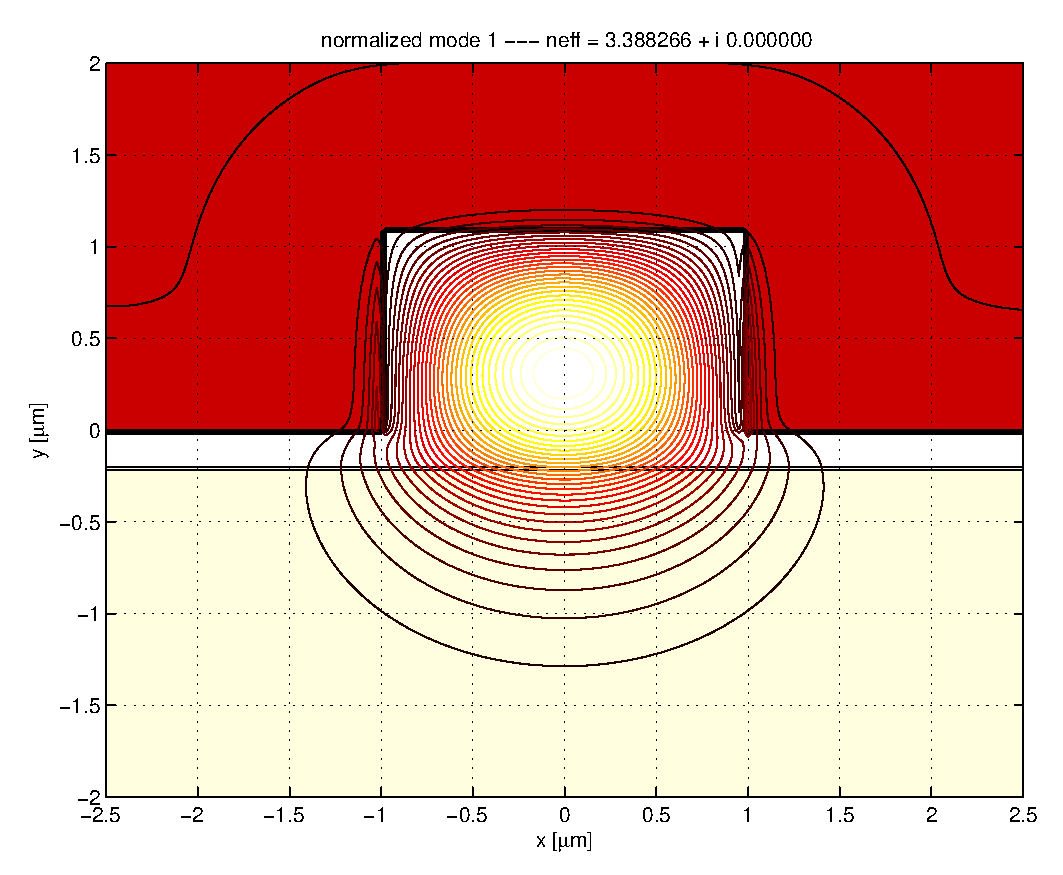
\includegraphics[width=5cm]{pics/wmm01_stern_TE1}}
    \subfigure[$TE_2$]{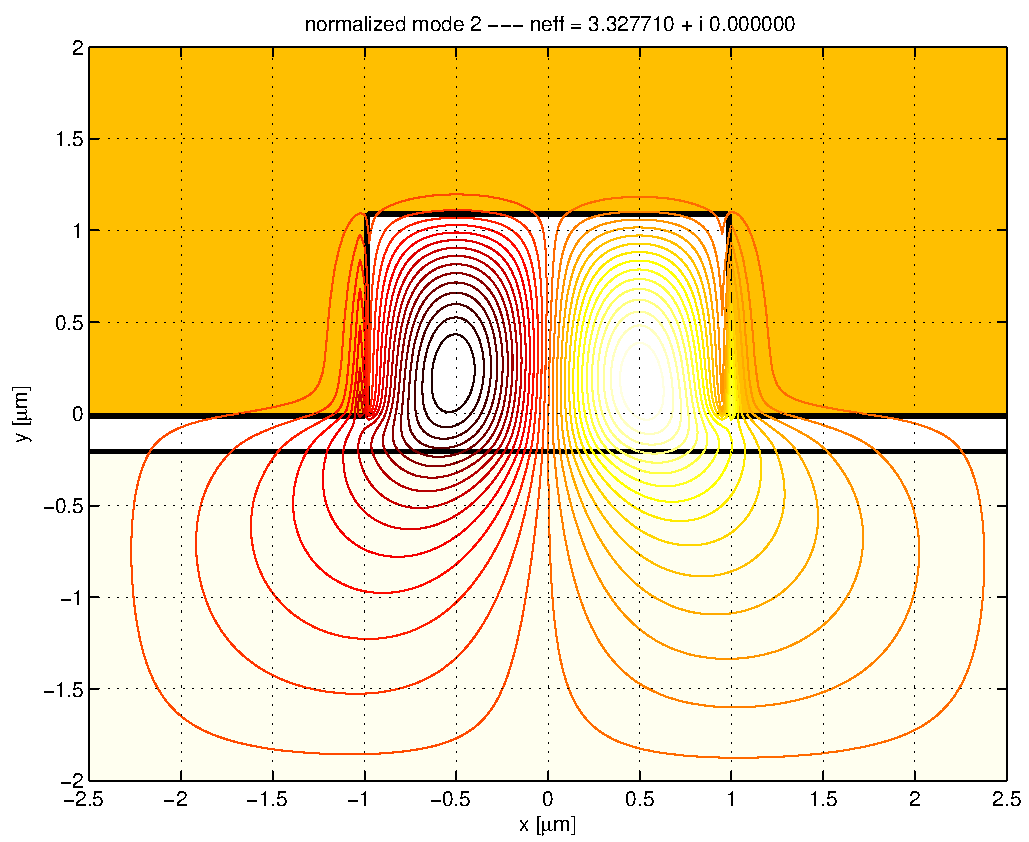
\includegraphics[width=5cm]{pics/wmm01_stern_TE2}}
    \subfigure[$TM_1$]{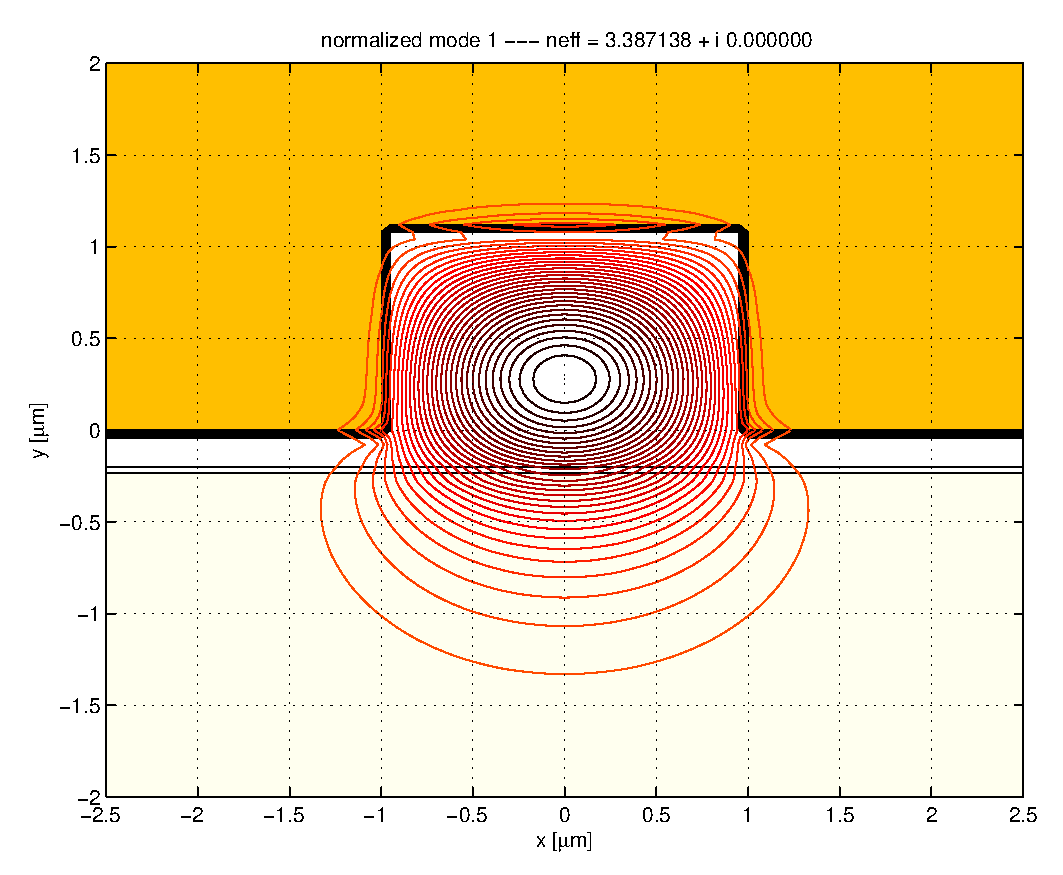
\includegraphics[width=5cm]{pics/wmm01_stern_TM1}}
    \subfigure[$TM_2$]{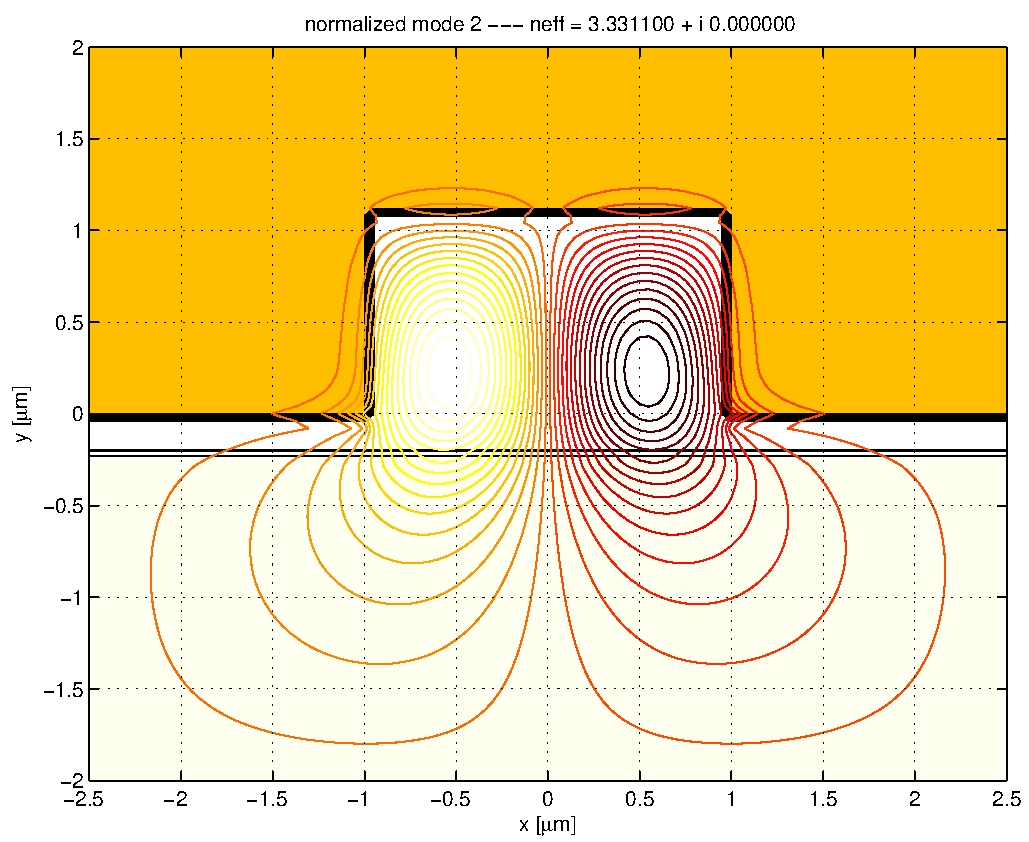
\includegraphics[width=5cm]{pics/wmm01_stern_TM2}}
  \end{center}
  \caption{Magnetic fields of the first four guided modes, computed by
    the semivectorial mode solver.}
  \label{fig:wmm1_stern}
\end{figure}  

\begin{figure}[htbp]
  \begin{center}
    \subfigure[$TE_1$]{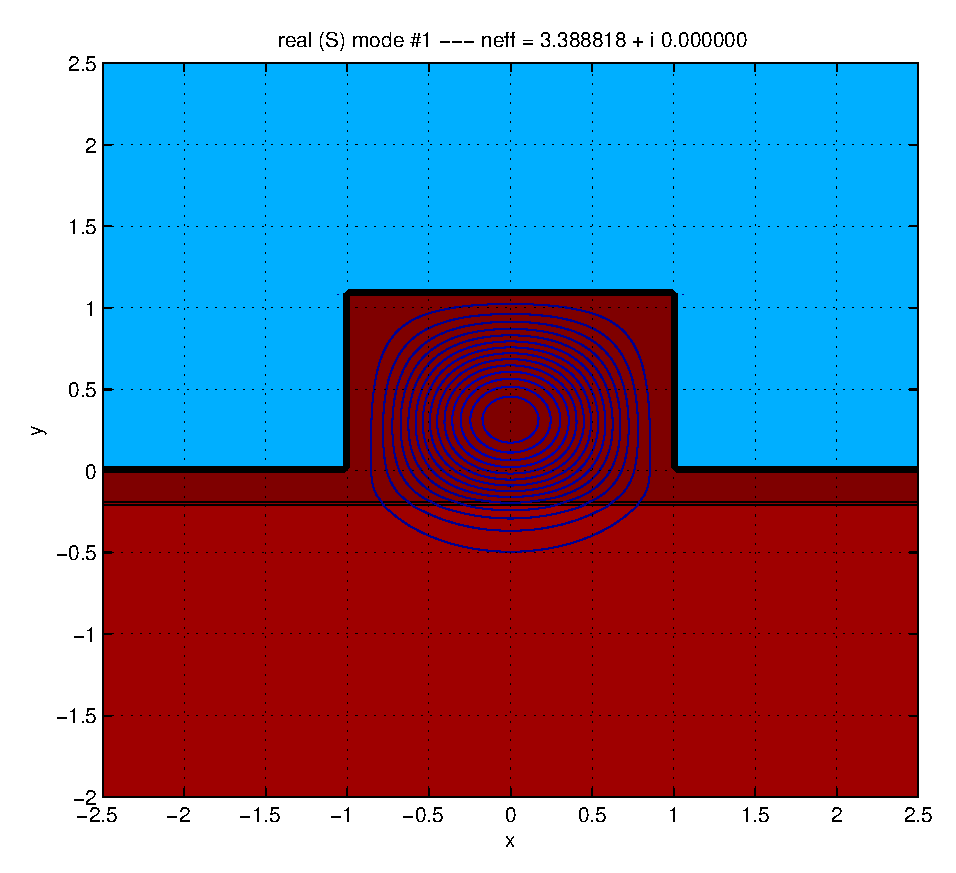
\includegraphics[width=5cm]{pics/wmm01_lusse_1}}
    \subfigure[$TE_2$]{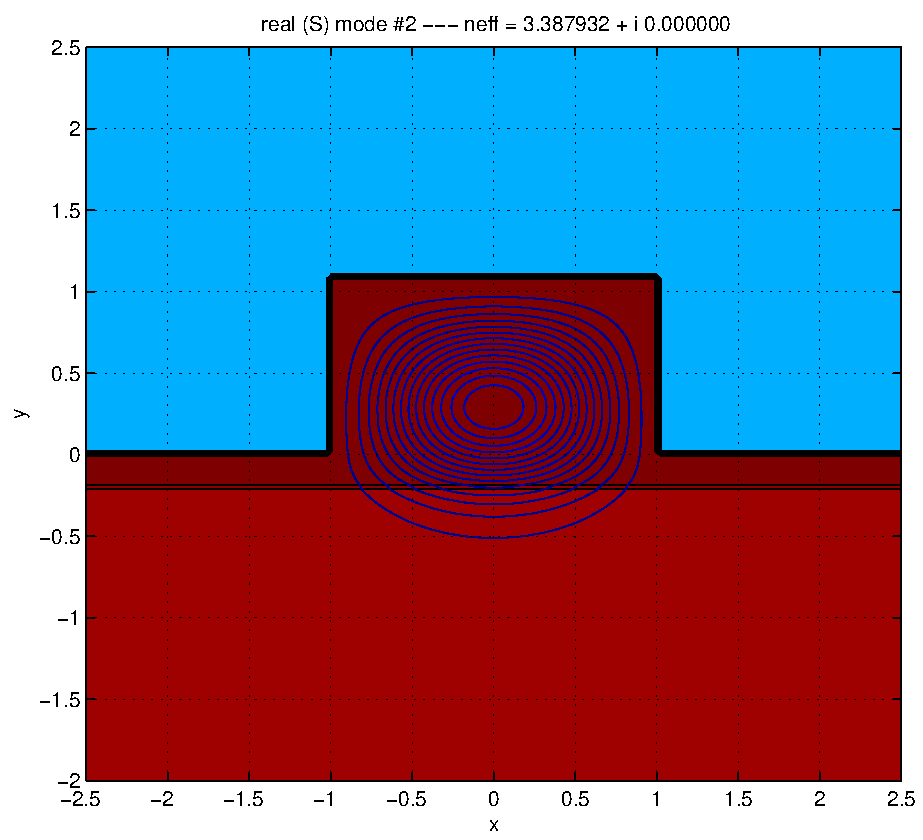
\includegraphics[width=5cm]{pics/wmm01_lusse_2}}
    \subfigure[$TM_1$]{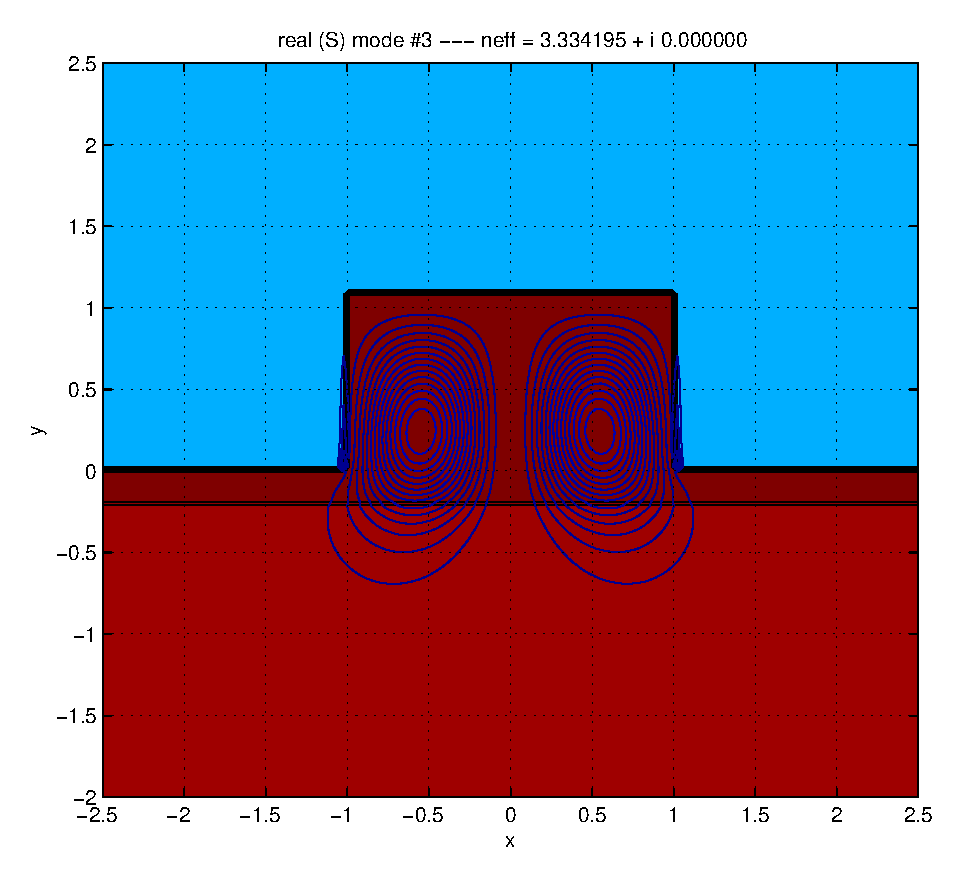
\includegraphics[width=5cm]{pics/wmm01_lusse_3}}
    \subfigure[$TM_2$]{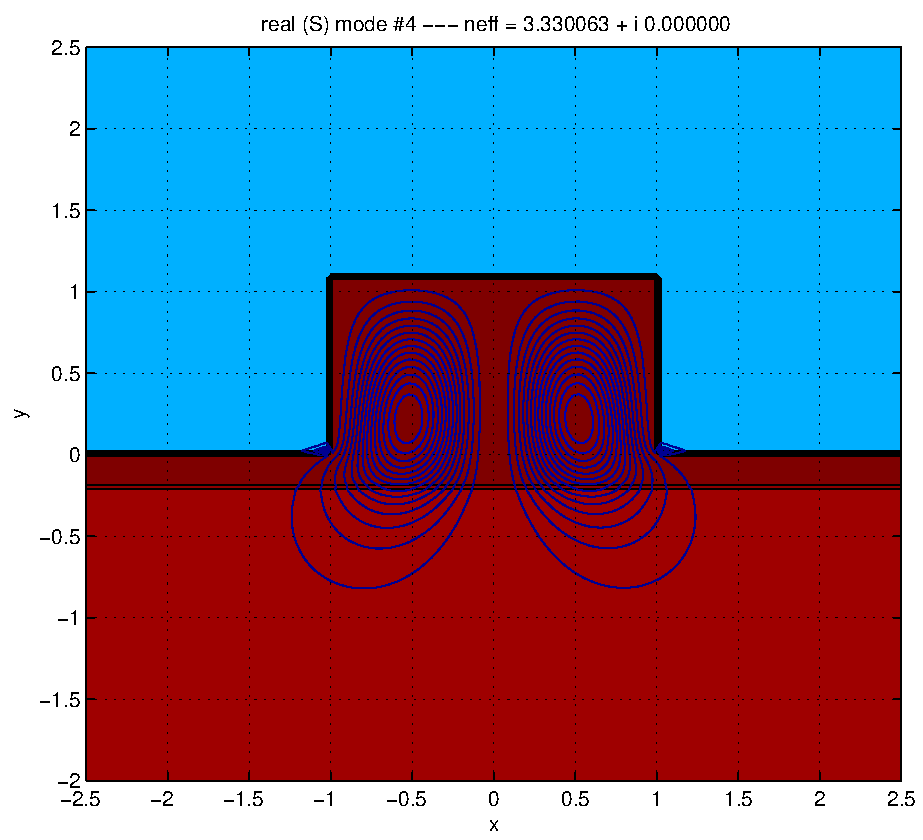
\includegraphics[width=5cm]{pics/wmm01_lusse_4}}
  \end{center}
  \caption{Longitudinal component of the Poynting vector of the first
    four guided modes, computed by the vectorial mode solver.}
  \label{fig:wmm1_lusse}
\end{figure}  

In this example, agreement between the semivectorial and the vectorial
mode solver is very good: it could make the Reader think that the two
algorithms are equivalent and the results are \emph{always}
similar. This is not true. It only happens because, for the particular
choice of the waveguide's structure, the guided
modes, even if not purely TE nor TM, are \emph{strongly} quasi-TE and
quasi-TM, with very small longitudinal $E_z$ and $H_z$ components:
ignoring them is a very small approximation.

In the next example, a waveguide is studied, where a fully vectorial
mode solver is needed. The device is shown in \figref{fig:plabs}. It
is a buried rectangular waveguide of $Si$ ($n_{core} = 3.45$) in
$SiO_2$ ($n_{cladding} = 1.445$), with $w = 500 nm$ and $h = 220 nm$.

\begin{figure}[htbp]
  \begin{center}
    \resizebox{4cm}{!}{\input{pics/plabs.pdf_t}}
  \end{center}
  \caption{Buried rectangular waveguide profile.}
  \label{fig:plabs}
\end{figure}

\tabref{tab:plabs} shows the results obtained with the two
algorithms. They differ greatly. In particular, the results given by
the semivectorial mode solver are definitely inaccurate: it predicts
that all the four modes are guided, instead of only the first two TE and
the first TM modes \cite{plabs}: this is correctly predicted by the
vectorial mode solver.

\begin{table}[htbp]
  \begin{center}
    \begin{tabular}{*{5}{c}}
      \hline
      & $TE_1$ & $TE_2$ & $TM_1$ & $TM_2$ \\
      \hline
      Semivectorial & 2.633596 & 2.263625 & 2.532738 & 1.976528 \\
      Vectorial & 2.446252 & 1.525369 & 1.800634 & 1.333947 \\
      \hline
    \end{tabular}
  \end{center}
  \caption{Effective indices\index{Effective!index|fig} for the first four modes of the buried
    rectangular waveguide in \figref{fig:plabs}, computed by both the
    semivectorial and vectorial mode solvers. Note that the $TM_2$ mode
    is guided for the semivectorial mode solver and not guided for the
    vectorial: the semivectorial is wrong.}
  \label{tab:plabs}
\end{table}

\begin{figure}[htbp]
  \begin{center}
    \subfigure[First TE mode: magnetic field.]{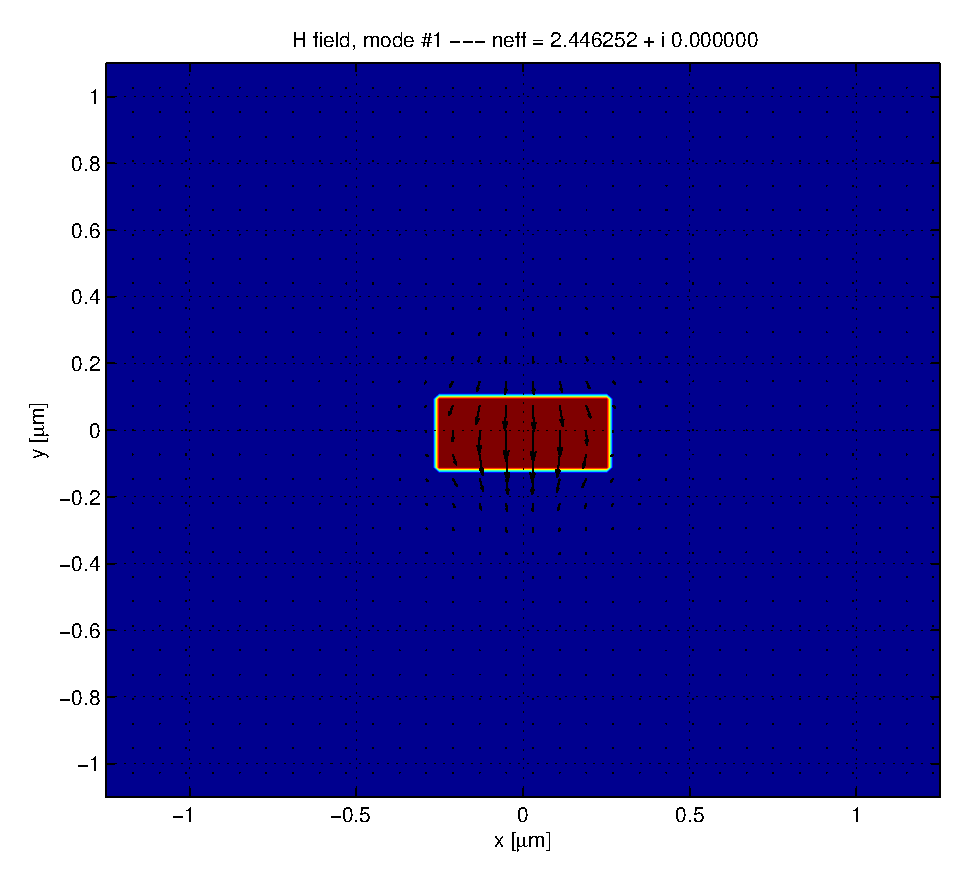
\includegraphics[width=5cm]{pics/plabs_TE1}}
    \subfigure[First TE mode: contour plot of the $H_y$ component.]{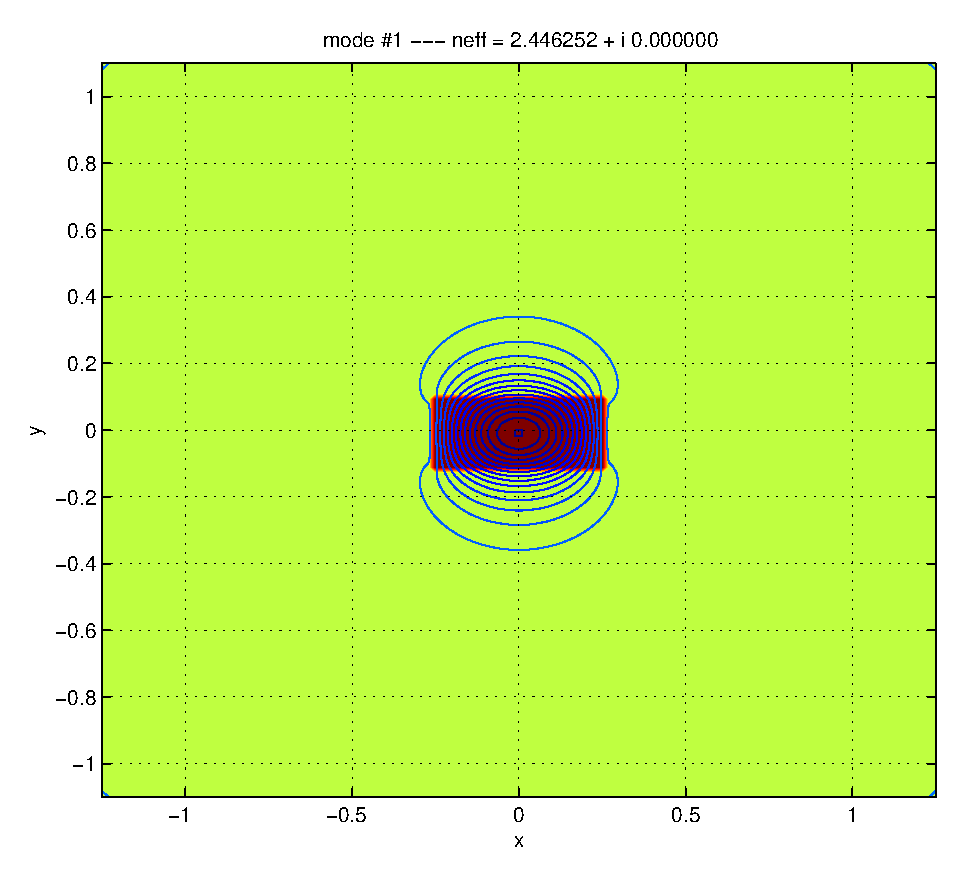
\includegraphics[width=5cm]{pics/plabs_TE1_contour}}
    \subfigure[First TM mode: magnetic field.]{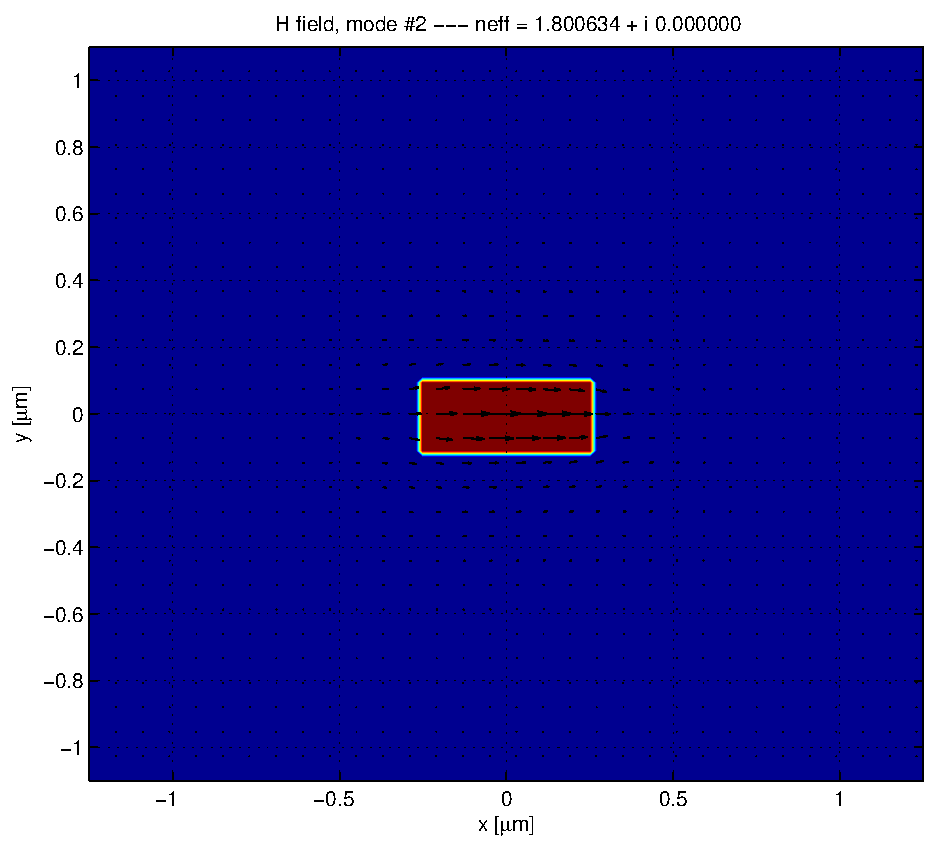
\includegraphics[width=5cm]{pics/plabs_TM1}}
    \subfigure[First TM mode: contour plot of the $H_x$ component.]{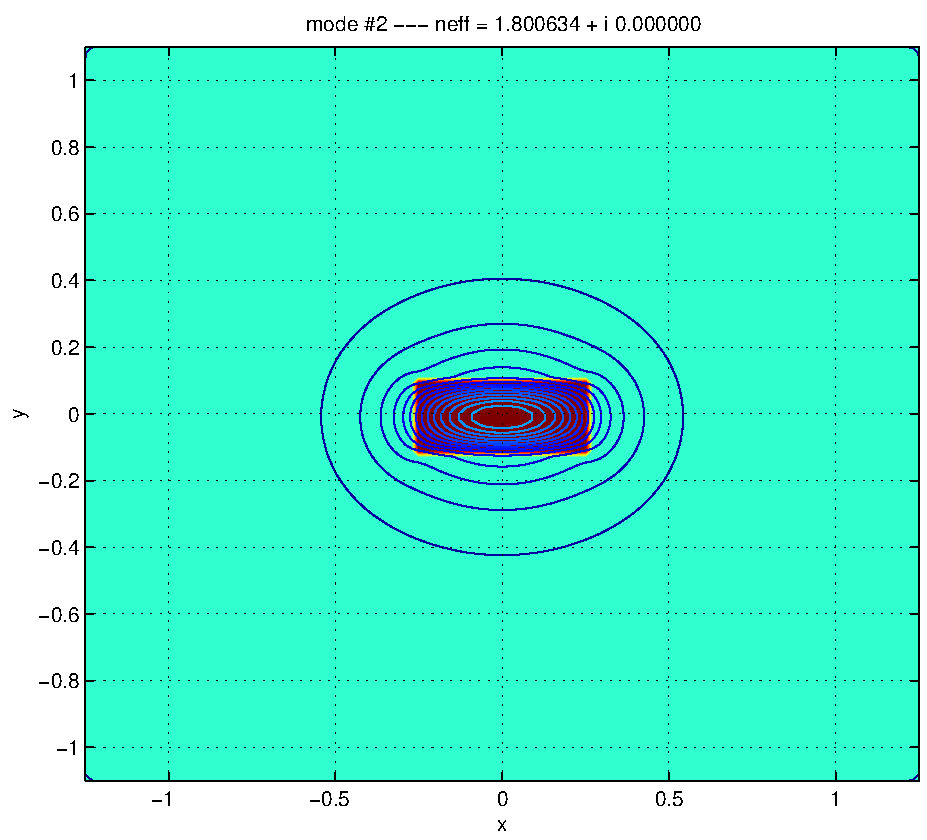
\includegraphics[width=5cm]{pics/plabs_TM1_contour}}
  \end{center}
  \caption{Magnetic field for the first two guided modes for the
  device in \figref{fig:plabs}.}
  \label{fig:plabs_field}
\end{figure}  

\figref{fig:plabs_field} shows the magnetic field for the first two
guided modes of the device.

More examples for the use of the vectorial mode solver can be found in
\charef{cha:polrot}.

\index{Finite Difference Method|)}

%% \OKKIO{fare degli esempi per la convergenza...}
%% \OKKIO{usare FIMMWAVE come reference??}
